\chapter{Matrimonial Projects}

The day following this scene, at the hour Debray usually chose to pay a
visit to Madame Danglars on his way to his office, his \textit{coupé} did not
appear. At this time, that is, about half-past twelve, Madame Danglars
ordered her carriage, and went out. Danglars, hidden behind a curtain,
watched the departure he had been waiting for. He gave orders that he
should be informed as soon as Madame Danglars appeared; but at two
o’clock she had not returned. He then called for his horses, drove to
the Chamber, and inscribed his name to speak against the budget. From
twelve to two o’clock Danglars had remained in his study, unsealing his
dispatches, and becoming more and more sad every minute, heaping figure
upon figure, and receiving, among other visits, one from Major
Cavalcanti, who, as stiff and exact as ever, presented himself
precisely at the hour named the night before, to terminate his business
with the banker.

On leaving the Chamber, Danglars, who had shown violent marks of
agitation during the sitting, and been more bitter than ever against
the ministry, re-entered his carriage, and told the coachman to drive
to the Avenue des Champs-Élysées, No. 30.

Monte Cristo was at home; only he was engaged with someone and begged
Danglars to wait for a moment in the drawing-room. While the banker was
waiting in the anteroom, the door opened, and a man dressed as an abbé
and doubtless more familiar with the house than he was, came in and
instead of waiting, merely bowed, passed on to the farther apartments,
and disappeared.

A minute after the door by which the priest had entered reopened, and
Monte Cristo appeared.

“Pardon me,” said he, “my dear baron, but one of my friends, the Abbé
Busoni, whom you perhaps saw pass by, has just arrived in Paris; not
having seen him for a long time, I could not make up my mind to leave
him sooner, so I hope this will be sufficient reason for my having made
you wait.”

“Nay,” said Danglars, “it is my fault; I have chosen my visit at a
wrong time, and will retire.”

“Not at all; on the contrary, be seated; but what is the matter with
you? You look careworn; really, you alarm me. Melancholy in a
capitalist, like the appearance of a comet, presages some misfortune to
the world.”

“I have been in ill-luck for several days,” said Danglars, “and I have
heard nothing but bad news.”

“Ah, indeed?” said Monte Cristo. “Have you had another fall at the
Bourse?”

“No; I am safe for a few days at least. I am only annoyed about a
bankrupt of Trieste.”

“Really? Does it happen to be Jacopo Manfredi?”

“Exactly so. Imagine a man who has transacted business with me for I
don’t know how long, to the amount of 800,000 or 900,000 francs during
the year. Never a mistake or delay—a fellow who paid like a prince.
Well, I was a million in advance with him, and now my fine Jacopo
Manfredi suspends payment!”

“Really?”

“It is an unheard-of fatality. I draw upon him for 600,000 francs, my
bills are returned unpaid, and, more than that, I hold bills of
exchange signed by him to the value of 400,000 francs, payable at his
correspondent’s in Paris at the end of this month. Today is the 30th. I
present them; but my correspondent has disappeared. This, with my
Spanish affairs, made a pretty end to the month.”

“Then you really lost by that affair in Spain?”

“Yes; only 700,000 francs out of my cash box—nothing more!”

“Why, how could you make such a mistake—such an old stager?”

“Oh, it is all my wife’s fault. She dreamed Don Carlos had returned to
Spain; she believes in dreams. It is magnetism, she says, and when she
dreams a thing it is sure to happen, she assures me. On this conviction
I allow her to speculate, she having her bank and her stockbroker; she
speculated and lost. It is true she speculates with her own money, not
mine; nevertheless, you can understand that when 700,000 francs leave
the wife’s pocket, the husband always finds it out. But do you mean to
say you have not heard of this? Why, the thing has made a tremendous
noise.”

“Yes, I heard it spoken of, but I did not know the details, and then no
one can be more ignorant than I am of the affairs in the Bourse.”

\begin{figure}[ht]
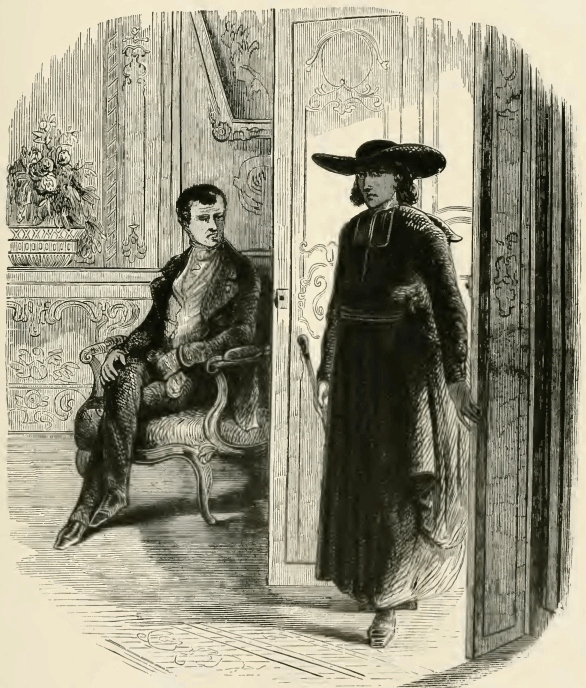
\includegraphics[width=\textwidth]{30251m.jpg}
\end{figure}

“Then you do not speculate?”

“I?—How could I speculate when I already have so much trouble in
regulating my income? I should be obliged, besides my steward, to keep
a clerk and a boy. But touching these Spanish affairs, I think that the
baroness did not dream the whole of the Don Carlos matter. The papers
said something about it, did they not?”

“Then you believe the papers?”

“I?—not the least in the world; only I fancied that the honest
\textit{Messager} was an exception to the rule, and that it only announced
telegraphic despatches.”

“Well, that’s what puzzles me,” replied Danglars; “the news of the
return of Don Carlos was brought by telegraph.”

“So that,” said Monte Cristo, “you have lost nearly 1,700,000 francs
this month.”

“Not nearly, indeed; that is exactly my loss.”

“\textit{Diable!}” said Monte Cristo compassionately, “it is a hard blow for a
third-rate fortune.”

“Third-rate,” said Danglars, rather humble, “what do you mean by that?”

“Certainly,” continued Monte Cristo, “I make three assortments in
fortune—first-rate, second-rate, and third-rate fortunes. I call those
first-rate which are composed of treasures one possesses under one’s
hand, such as mines, lands, and funded property, in such states as
France, Austria, and England, provided these treasures and property
form a total of about a hundred millions; I call those second-rate
fortunes, that are gained by manufacturing enterprises, joint-stock
companies, viceroyalties, and principalities, not drawing more than
1,500,000 francs, the whole forming a capital of about fifty millions;
finally, I call those third-rate fortunes, which are composed of a
fluctuating capital, dependent upon the will of others, or upon chances
which a bankruptcy involves or a false telegram shakes, such as banks,
speculations of the day—in fact, all operations under the influence of
greater or less mischances, the whole bringing in a real or fictitious
capital of about fifteen millions. I think this is about your position,
is it not?”

“Confound it, yes!” replied Danglars.

“The result, then, of six more such months as this would be to reduce
the third-rate house to despair.”

“Oh,” said Danglars, becoming very pale, how you are running on!”

“Let us imagine seven such months,” continued Monte Cristo, in the same
tone. “Tell me, have you ever thought that seven times 1,700,000 francs
make nearly twelve millions? No, you have not;—well, you are right, for
if you indulged in such reflections, you would never risk your
principal, which is to the speculator what the skin is to civilized
man. We have our clothes, some more splendid than others,—this is our
credit; but when a man dies he has only his skin; in the same way, on
retiring from business, you have nothing but your real principal of
about five or six millions, at the most; for third-rate fortunes are
never more than a fourth of what they appear to be, like the locomotive
on a railway, the size of which is magnified by the smoke and steam
surrounding it. Well, out of the five or six millions which form your
real capital, you have just lost nearly two millions, which must, of
course, in the same degree diminish your credit and fictitious fortune;
to follow out my simile, your skin has been opened by bleeding, and
this if repeated three or four times will cause death—so pay attention
to it, my dear Monsieur Danglars. Do you want money? Do you wish me to
lend you some?”

\begin{figure}[ht]
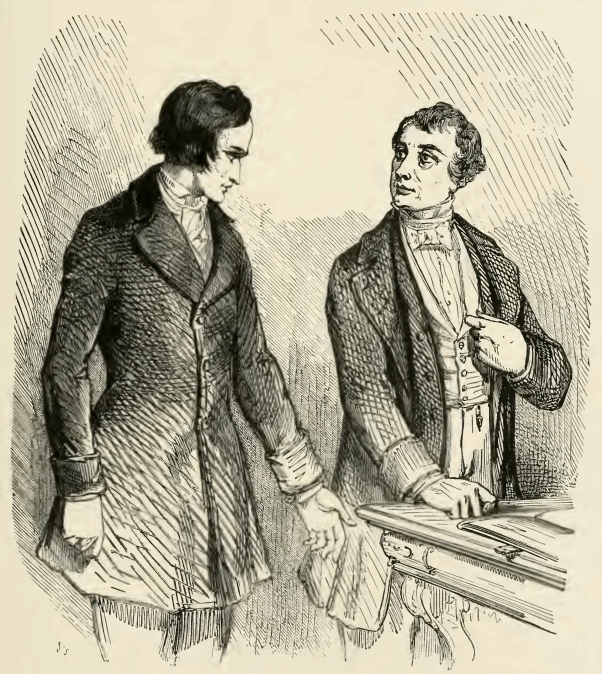
\includegraphics[width=\textwidth]{30253m.jpg}
\end{figure}

“What a bad calculator you are!” exclaimed Danglars, calling to his
assistance all his philosophy and dissimulation. “I have made money at
the same time by speculations which have succeeded. I have made up the
loss of blood by nutrition. I lost a battle in Spain, I have been
defeated in Trieste, but my naval army in India will have taken some
galleons, and my Mexican pioneers will have discovered some mine.”

“Very good, very good! But the wound remains and will reopen at the
first loss.”

“No, for I am only embarked in certainties,” replied Danglars, with the
air of a mountebank sounding his own praises; “to involve me, three
governments must crumble to dust.”

“Well, such things have been.”

“That there should be a famine!”

“Recollect the seven fat and the seven lean kine.”

“Or, that the sea should become dry, as in the days of Pharaoh, and
even then my vessels would become caravans.”

“So much the better. I congratulate you, my dear M. Danglars,” said
Monte Cristo; “I see I was deceived, and that you belong to the class
of second-rate fortunes.”

“I think I may aspire to that honor,” said Danglars with a smile, which
reminded Monte Cristo of the sickly moons which bad artists are so fond
of daubing into their pictures of ruins. “But, while we are speaking of
business,” Danglars added, pleased to find an opportunity of changing
the subject, “tell me what I am to do for M. Cavalcanti.”

“Give him money, if he is recommended to you, and the recommendation
seems good.”

“Excellent; he presented himself this morning with a bond of 40,000
francs, payable at sight, on you, signed by Busoni, and returned by you
to me, with your endorsement—of course, I immediately counted him over
the forty bank-notes.”

Monte Cristo nodded his head in token of assent.

“But that is not all,” continued Danglars; “he has opened an account
with my house for his son.”

“May I ask how much he allows the young man?”

“Five thousand francs per month.”

“Sixty thousand francs per year. I thought I was right in believing
that Cavalcanti to be a stingy fellow. How can a young man live upon
5,000 francs a month?”

“But you understand that if the young man should want a few thousands
more——”

“Do not advance it; the father will never repay it. You do not know
these ultramontane millionaires; they are regular misers. And by whom
were they recommended to you?”

“Oh, by the house of Fenzi, one of the best in Florence.”

“I do not mean to say you will lose, but, nevertheless, mind you hold
to the terms of the agreement.”

“Would you not trust the Cavalcanti?”

“I? oh, I would advance ten millions on his signature. I was only
speaking in reference to the second-rate fortunes we were mentioning
just now.”

“And with all this, how unassuming he is! I should never have taken him
for anything more than a mere major.”

“And you would have flattered him, for certainly, as you say, he has no
manner. The first time I saw him he appeared to me like an old
lieutenant who had grown mouldy under his epaulets. But all the
Italians are the same; they are like old Jews when they are not
glittering in Oriental splendor.”

“The young man is better,” said Danglars.

“Yes; a little nervous, perhaps, but, upon the whole, he appeared
tolerable. I was uneasy about him.”

“Why?”

“Because you met him at my house, just after his introduction into the
world, as they told me. He has been travelling with a very severe
tutor, and had never been to Paris before.”

“Ah, I believe noblemen marry amongst themselves, do they not?” asked
Danglars carelessly; “they like to unite their fortunes.”

“It is usual, certainly; but Cavalcanti is an original who does nothing
like other people. I cannot help thinking that he has brought his son
to France to choose a wife.”

“Do you think so?”

“I am sure of it.”

“And you have heard his fortune mentioned?”

“Nothing else was talked of; only some said he was worth millions, and
others that he did not possess a farthing.”

“And what is your opinion?”

“I ought not to influence you, because it is only my own personal
impression.”

“Well, and it is that——”

“My opinion is, that all these old \textit{podestàs}, these ancient
\textit{condottieri},—for the Cavalcanti have commanded armies and governed
provinces,—my opinion, I say, is, that they have buried their millions
in corners, the secret of which they have transmitted only to their
eldest sons, who have done the same from generation to generation; and
the proof of this is seen in their yellow and dry appearance, like the
florins of the republic, which, from being constantly gazed upon, have
become reflected in them.”

“Certainly,” said Danglars, “and this is further supported by the fact
of their not possessing an inch of land.”

“Very little, at least; I know of none which Cavalcanti possesses,
excepting his palace in Lucca.”

“Ah, he has a palace?” said Danglars, laughing; “come, that is
something.”

“Yes; and more than that, he lets it to the Minister of Finance while
he lives in a simple house. Oh, as I told you before, I think the old
fellow is very close.”

“Come, you do not flatter him.”

“I scarcely know him; I think I have seen him three times in my life;
all I know relating to him is through Busoni and himself. He was
telling me this morning that, tired of letting his property lie dormant
in Italy, which is a dead nation, he wished to find a method, either in
France or England, of multiplying his millions, but remember, that
though I place great confidence in Busoni, I am not responsible for
this.”

“Never mind; accept my thanks for the client you have sent me. It is a
fine name to inscribe on my ledgers, and my cashier was quite proud of
it when I explained to him who the Cavalcanti were. By the way, this is
merely a simple question, when this sort of people marry their sons, do
they give them any fortune?”

“Oh, that depends upon circumstances. I know an Italian prince, rich as
a gold mine, one of the noblest families in Tuscany, who, when his sons
married according to his wish, gave them millions; and when they
married against his consent, merely allowed them thirty crowns a month.
Should Andrea marry according to his father’s views, he will, perhaps,
give him one, two, or three millions. For example, supposing it were
the daughter of a banker, he might take an interest in the house of the
father-in-law of his son; then again, if he disliked his choice, the
major takes the key, double-locks his coffer, and Master Andrea would
be obliged to live like the sons of a Parisian family, by shuffling
cards or rattling the dice.”

“Ah, that boy will find out some Bavarian or Peruvian princess; he will
want a crown, an El Dorado, and Potosí.”

“No; these grand lords on the other side of the Alps frequently marry
into plain families; like Jupiter, they like to cross the race. But do
you wish to marry Andrea, my dear M. Danglars, that you are asking so
many questions?”

“\textit{Ma foi},” said Danglars, “it would not be a bad speculation, I fancy,
and you know I am a speculator.”

“You are not thinking of Mademoiselle Danglars, I hope; you would not
like poor Andrea to have his throat cut by Albert?”

“Albert,” repeated Danglars, shrugging his shoulders; “ah, well; he
would care very little about it, I think.”

“But he is betrothed to your daughter, I believe?”

“Well, M. de Morcerf and I have talked about this marriage, but Madame
de Morcerf and Albert——”

“You do not mean to say that it would not be a good match?”

“Indeed, I imagine that Mademoiselle Danglars is as good as M. de
Morcerf.”

“Mademoiselle Danglars’ fortune will be great, no doubt, especially if
the telegraph should not make any more mistakes.”

“Oh, I do not mean her fortune only; but tell me——”

“What?”

“Why did you not invite M. and Madame de Morcerf to your dinner?”

“I did so, but he excused himself on account of Madame de Morcerf being
obliged to go to Dieppe for the benefit of sea air.”

“Yes, yes,” said Danglars, laughing, “it would do her a great deal of
good.”

“Why so?”

“Because it is the air she always breathed in her youth.”

Monte Cristo took no notice of this ill-natured remark.

“But still, if Albert be not so rich as Mademoiselle Danglars,” said
the count, “you must allow that he has a fine name?”

“So he has; but I like mine as well.”

“Certainly; your name is popular, and does honor to the title they have
adorned it with; but you are too intelligent not to know that according
to a prejudice, too firmly rooted to be exterminated, a nobility which
dates back five centuries is worth more than one that can only reckon
twenty years.”

“And for this very reason,” said Danglars with a smile, which he tried
to make sardonic, “I prefer M. Andrea Cavalcanti to M. Albert de
Morcerf.”

“Still, I should not think the Morcerfs would yield to the Cavalcanti?”

“The Morcerfs!—Stay, my dear count,” said Danglars; “you are a man of
the world, are you not?”

“I think so.”

“And you understand heraldry?”

“A little.”

“Well, look at my coat-of-arms, it is worth more than Morcerf’s.”

“Why so?”

“Because, though I am not a baron by birth, my real name is, at least,
Danglars.”

“Well, what then?”

“While his name is not Morcerf.”

“How?—not Morcerf?”

“Not the least in the world.”

“Go on.”

“I have been made a baron, so that I actually am one; he made himself a
count, so that he is not one at all.”

“Impossible!”

“Listen my dear count; M. de Morcerf has been my friend, or rather my
acquaintance, during the last thirty years. You know I have made the
most of my arms, though I never forgot my origin.”

“A proof of great humility or great pride,” said Monte Cristo.

“Well, when I was a clerk, Morcerf was a mere fisherman.”

“And then he was called——”

“Fernand.”

“Only Fernand?”

“Fernand Mondego.”

“You are sure?”

“\textit{Pardieu!} I have bought enough fish of him to know his name.”

“Then, why did you think of giving your daughter to him?”

“Because Fernand and Danglars, being both parvenus, both having become
noble, both rich, are about equal in worth, excepting that there have
been certain things mentioned of him that were never said of me.”

“What?”

“Oh, nothing!”

“Ah, yes; what you tell me recalls to mind something about the name of
Fernand Mondego. I have heard that name in Greece.”

“In conjunction with the affairs of Ali Pasha?”

“Exactly so.”

“This is the mystery,” said Danglars. “I acknowledge I would have given
anything to find it out.”

“It would be very easy if you much wished it?”

“How so?”

“Probably you have some correspondent in Greece?”

“I should think so.”

“At Yanina?”

“Everywhere.”

“Well, write to your correspondent in Yanina, and ask him what part was
played by a Frenchman named Fernand Mondego in the catastrophe of Ali
Tepelini.”

“You are right,” exclaimed Danglars, rising quickly, “I will write
today.”

“Do so.”

“I will.”

\begin{figure}[ht]
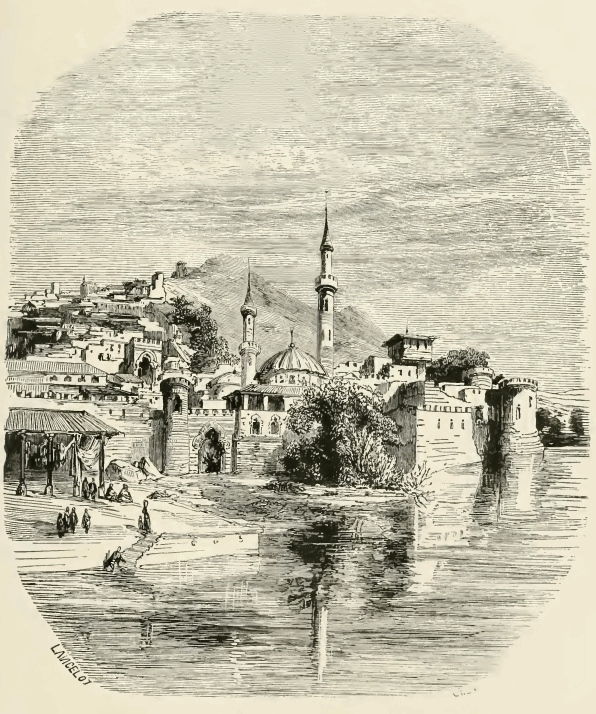
\includegraphics[width=\textwidth]{30259m.jpg}
\end{figure}

“And if you should hear of anything very scandalous——”

“I will communicate it to you.”

“You will oblige me.”

Danglars rushed out of the room, and made but one leap into his
\textit{coupé}.
